\documentclass[UTF8,a4paper,11pt,fontset=fandol]{ctexart}
\usepackage[margin=19mm,headheight=15pt]{geometry}
\usepackage{graphicx,xcolor,booktabs,tabularx,array,fancyhdr,float,caption,listings,tikz,amsmath,amssymb}
\usetikzlibrary{arrows.meta,positioning}
\usepackage[colorlinks=true,linkcolor=sea,urlcolor=sea,citecolor=sea]{hyperref}

% 调色板与排版细节定义
\definecolor{sea}{HTML}{146679}
\definecolor{ink}{HTML}{23343E}
\definecolor{pale}{HTML}{EDF4F6}
\definecolor{muted}{HTML}{61727B}
\definecolor{darksea}{HTML}{0D4552}
\definecolor{border}{HTML}{D1E2E6}

\setlength{\parindent}{2em}
\setlength{\parskip}{2.5pt}
\linespread{1.12}

\ctexset{
  section={format=\Large\bfseries\color{sea}},
  subsection={format=\normalsize\bfseries\color{ink}},
  subsubsection={format=\small\bfseries\color{darksea}}
}

\captionsetup{font=small,labelfont=bf,textfont={color=muted},skip=5pt}

\pagestyle{fancy}\fancyhf{}
\fancyhead[L]{\small\color{muted}空海 · 无人机、无人艇与海洋工程环境素材库技术白皮书}
\fancyhead[R]{\small\color{muted}2026.10.24}
\fancyfoot[C]{\small\color{muted}\thepage}
\renewcommand{\headrulewidth}{0.3pt}

\hypersetup{
  pdftitle={空海：跨介质无人载具、海洋工程环境与协同算法库综合技术白皮书},
  pdfauthor={朱华天, Gemini 3.8 Flash, GPT-6 Astra}
}

\lstset{
  basicstyle=\ttfamily\footnotesize,
  breaklines=true,
  columns=fullflexible,
  frame=single,
  rulecolor=\color{border},
  backgroundcolor=\color{pale},
  showstringspaces=false,
  xleftmargin=6pt,
  xrightmargin=6pt,
  aboveskip=5pt,
  belowskip=5pt
}

\newcommand{\shot}[3]{%
  \begin{figure}[htbp]
    \centering
    \includegraphics[width=#2\linewidth]{images/#1}
    \caption{#3}
  \end{figure}
}
\newcommand{\repo}{https://github.com/ZHT1235456/air-water-3d-asset-library}

\begin{document}
\thispagestyle{empty}

{\color{sea}\small TECHNICAL WHITE PAPER \quad / \quad THREE.JS + VITE + TYPESCRIPT}
\vspace{3mm}

\begin{center}
{\Huge\bfseries\color{ink}空\quad 海}\\[3.5mm]
{\LARGE\bfseries 跨介质无人载具、海洋工程环境与协同算法库}\\[2.5mm]
{\large 综合技术白皮书与系统演进日志}\\[4.5mm]
{\large 朱华天，Gemini 3.8 Flash，GPT-6 Astra}\\[3mm]
{\large 2026年10月24日}\\[1.5mm]
{\small\url{https://github.com/ZHT1235456/air-water-3d-asset-library}}
\end{center}

\vspace{1mm}
\begin{figure}[H]
  \centering
  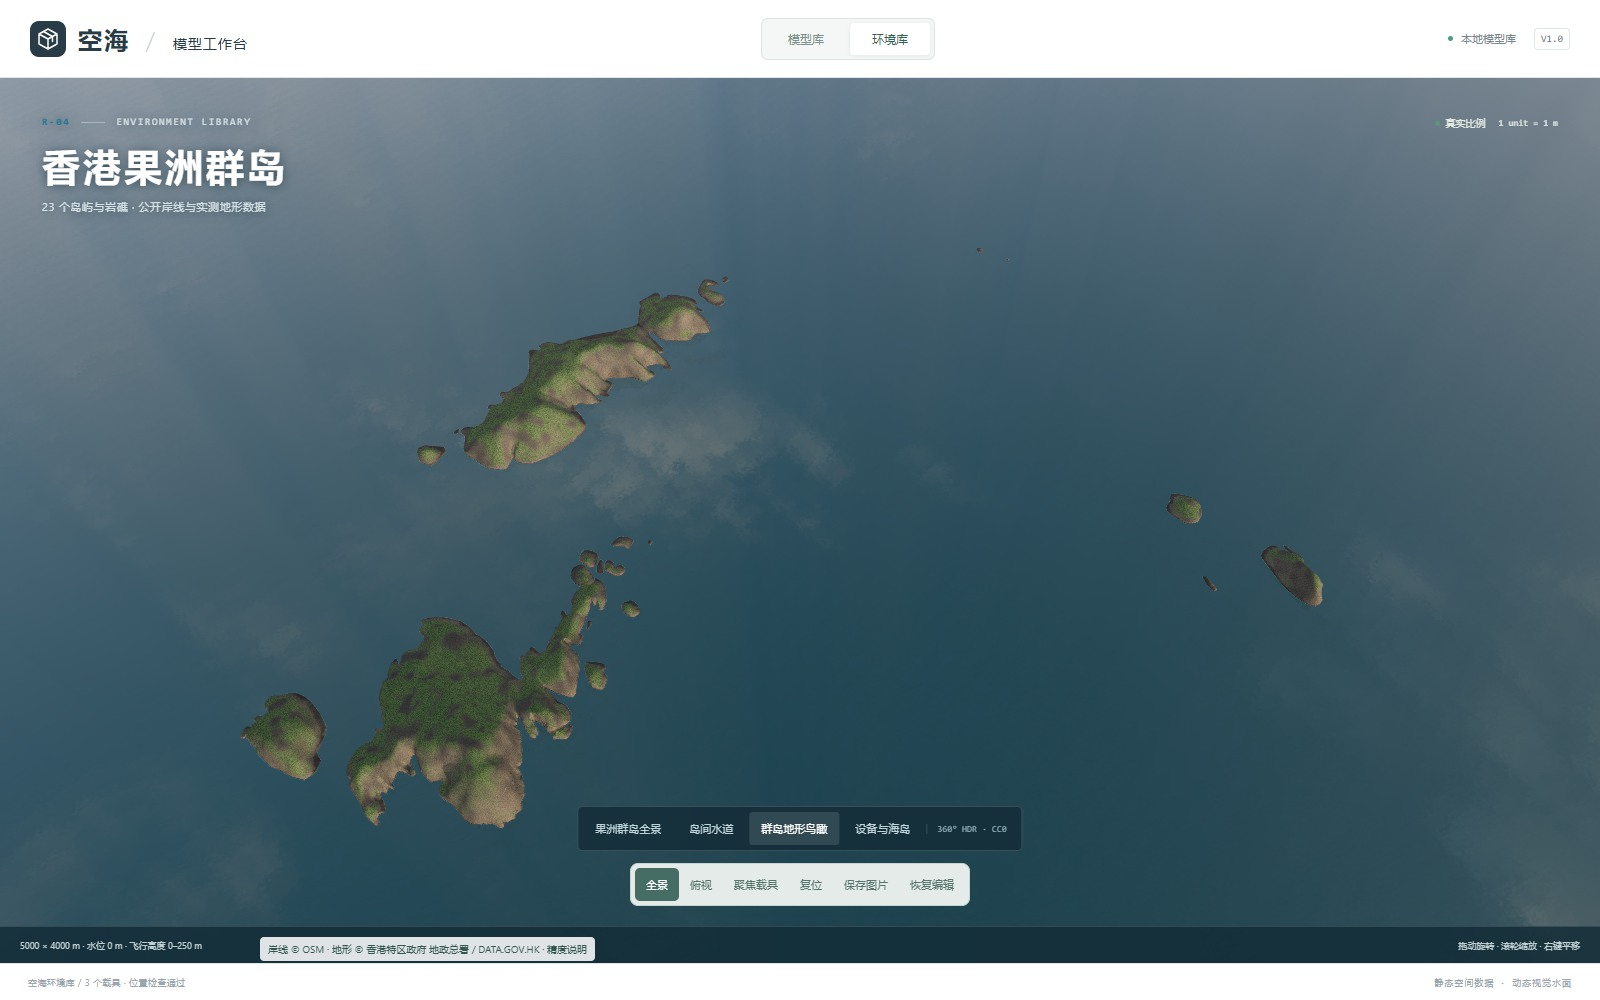
\includegraphics[width=0.98\linewidth]{images/ninepin-aerial.jpg}
  \caption{香港果洲群岛宏观鸟瞰：真实闭合岸线、5米高程网格与动态实时海面渲染的综合呈现。}
\end{figure}

\vspace{-1mm}
\noindent\colorbox{pale}{\parbox{\dimexpr\linewidth-2\fboxsep}{%
\vspace{1.5mm}
\textbf{摘要}\quad 本项目构建了一套纯代码生成、高度轻量化且具备严密拓扑与物理几何约束的跨介质无人装备三维素材库、多尺度实景水域工程环境与多艇协同算法库。系统基于现代 WebGL（Three.js r180 / Vite 8 / TypeScript 5.9），全面扩展实现了包含 8 款四旋翼无人机与 10 款单尖船首无人艇（USV）的 18 款原创程序化模型；构建了由原创深水集装箱港工程示范、港珠澳大桥青州与九洲通航桥、北海 Hornsea 2 离岸风场、香港果洲群岛以及新增的杭州西湖三岛水域、新加坡加冷盆地、鹿特丹瓦尔港组成的 8 大实景地理水域体系；提出了基于 HDR 辐射度预过滤、对数深度缓冲（Logarithmic Depth Buffer）与平面镜像反射的物理对齐渲染管线；新增了涵盖 A*、Dijkstra、领航—跟随编队、分布式一致性与分区往复全覆盖的 5 项无人艇运动规划与集群协同实验，集成了基于连续运动扫掠圆的连续碰撞门（Continuous Collision Gate）机制。全系统 31 项自动化测试全量通过，在 Intel Arc 140V GPU 上实测保持 60 FPS 稳定帧率与零显存泄漏，为跨介质机器人控制与算法验证提供了高可靠的数字基座。\\[1mm]
\textbf{关键词}\quad 跨介质无人系统；程序化建模；单尖船首；实景水域；路径规划；编队协同；对数深度缓冲
\vspace{1.5mm}
}}

\vfill
\noindent{\small\color{muted}声明：本文署名依照项目发起者与协作团队要求列示。文中所附渲染截图均来自浏览器内实时渲染捕获；第三方天空辐射度数据、OpenStreetMap 矢量地理数据与香港特区政府地政总署数字地形模型之法定授权在文末及仓库台账中严格注明。}
\clearpage

\section{系统总体架构与跨介质设计哲学}

在跨介质无人系统（空海装备协同）仿真与算法验证中，传统 3D 资产普遍存在“几何拓扑松散、尺度脱离实际、场景与算法强耦合、运行时开销庞大”等局限。本项目从严密的数学拓扑和物理约束出发，基于现代 Web 技术栈构建了高内聚、低耦合的系统架构。

\subsection{软件工程分层解耦体系}
系统在工程层面划分为五个高度正交的子系统：
\begin{enumerate}
  \item \textbf{参数化运载器建模层（\texttt{src/models/}）}：基于解析曲面生成 18 款无人机与无人艇几何，提供独立生命周期与部件映射；
  \item \textbf{语义拓扑空间层（\texttt{src/environments/spatial.ts}）}：维护形式化水域边界、障碍物垂直区间与安全出生点，支持纯数据无头快速判定；
  \item \textbf{工程环境与渲染管线层（\texttt{src/environments/}）}：集成实景地理高程网格、实例化工程设施、HDR 辐射度环境与对数深度缓冲海面；
  \item \textbf{无人艇协同与运动规划算法层（\texttt{src/algorithms/}）}：提供 A*、Dijkstra、领航跟随、一致性与全覆盖算法，支持 Web Worker 异步多线程求解；
  \item \textbf{交互工作台与状态沙盒（\texttt{src/scenes/editor.ts}）}：实现轨道控制、多机位切换、参数调节、轨迹回看与版本化 JSON 序列化热插拔。
\end{enumerate}

\begin{figure}[htbp]\centering
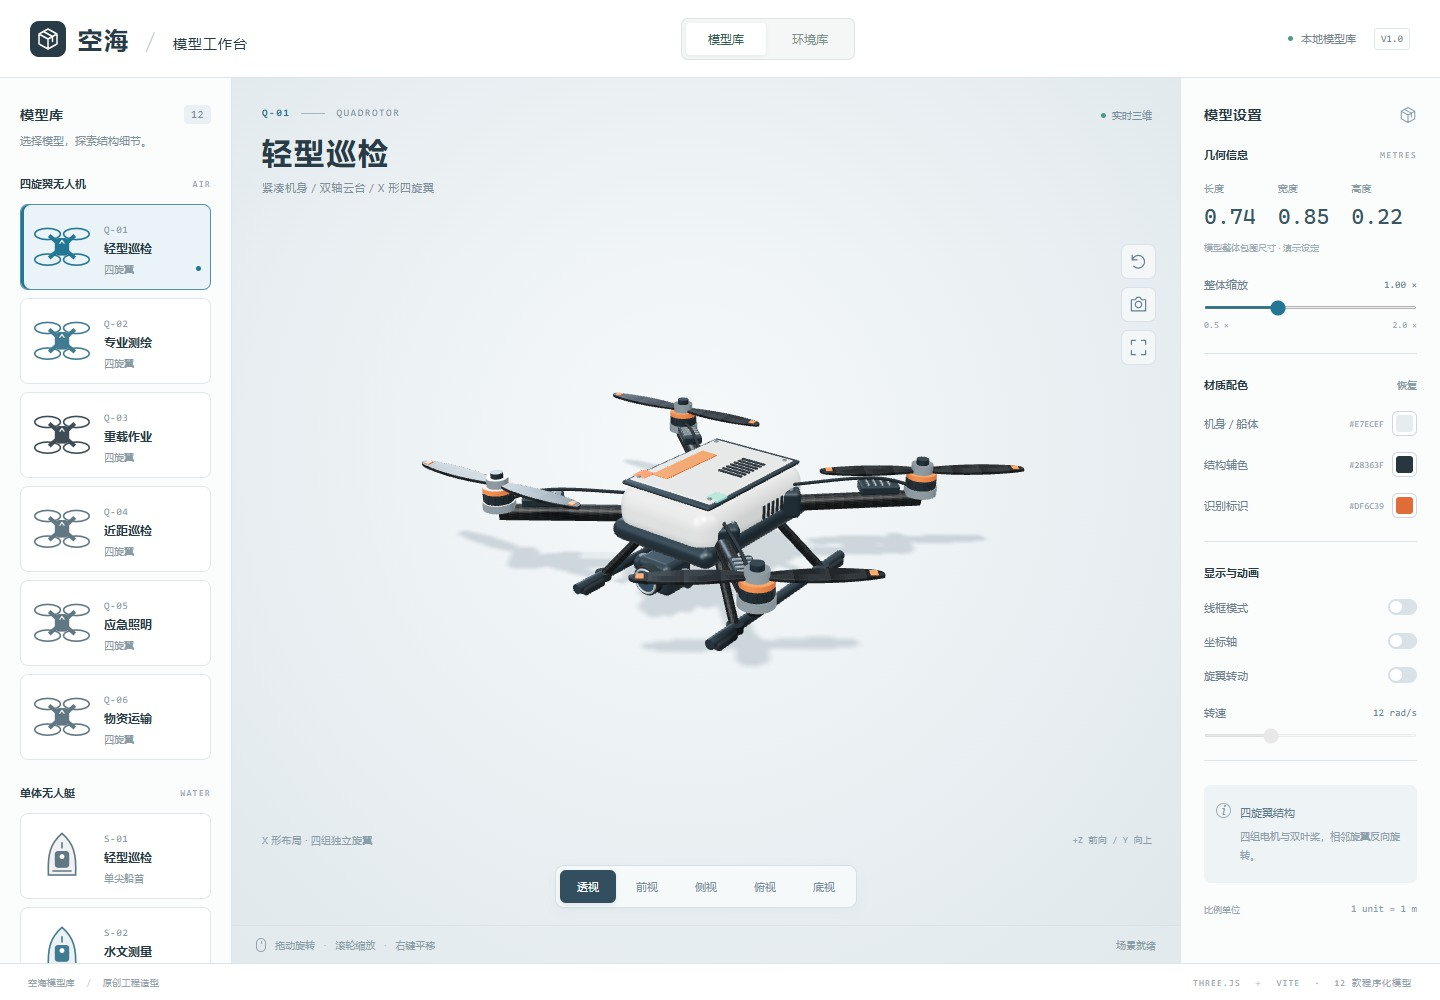
\includegraphics[width=.49\linewidth]{images/quadrotor.jpg}\hfill
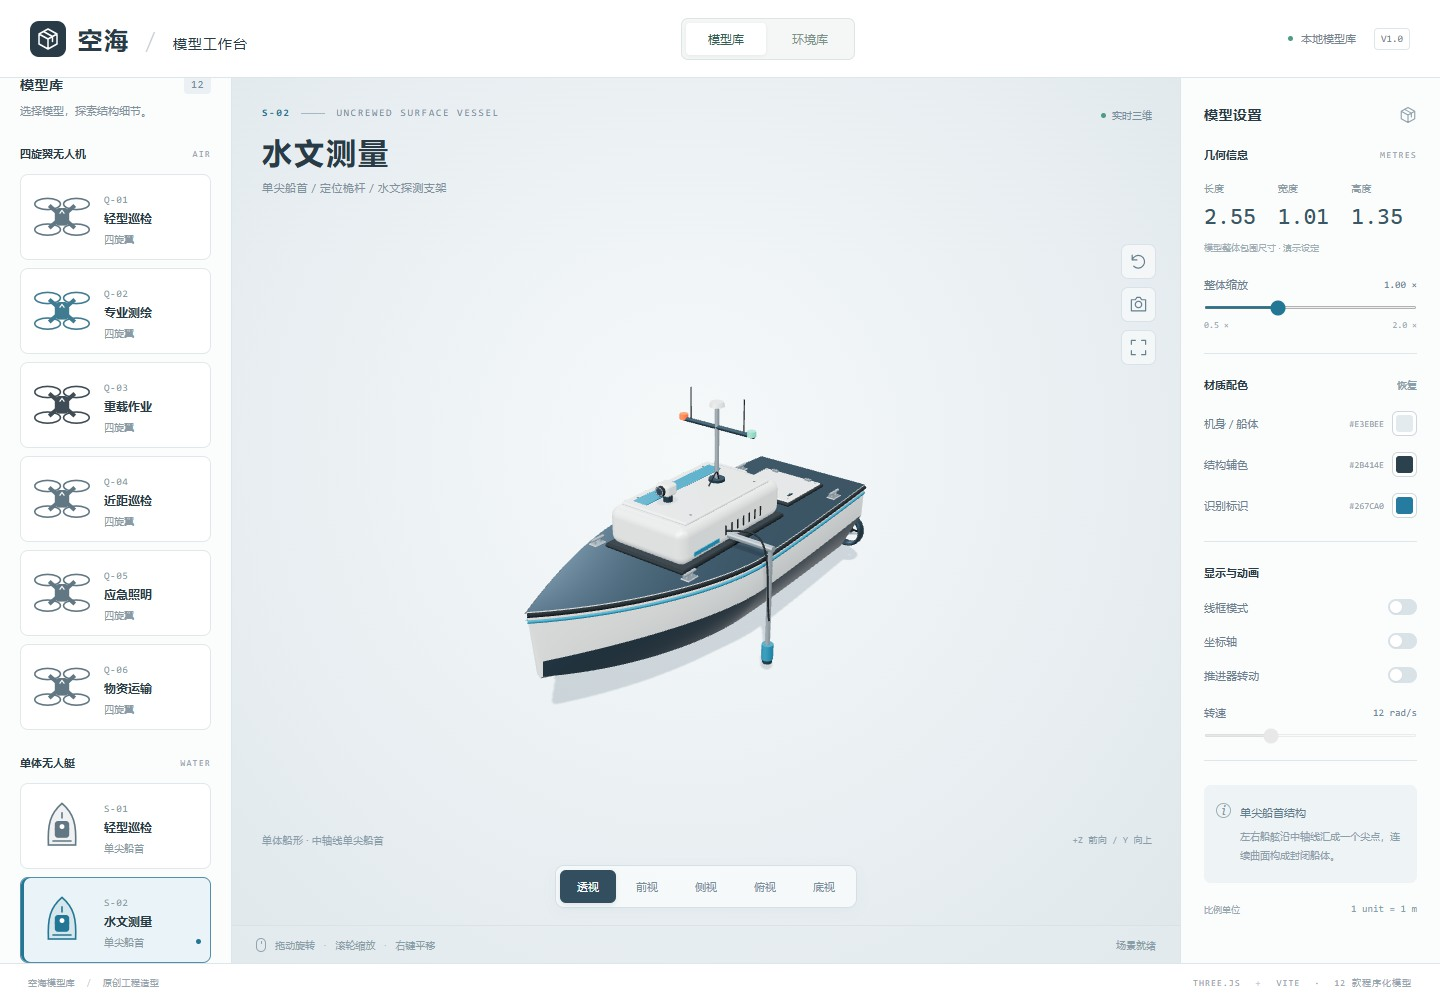
\includegraphics[width=.49\linewidth]{images/usv.jpg}
\caption{轻型巡检四旋翼无人机与水文测量无人艇。色彩方案、尺寸尺度、构件层级及生命周期接口均由代码闭环管理。}
\end{figure}

\subsection{绝对坐标系统与跨介质物理基准面}
系统全局严格遵循右手笛卡尔米制世界坐标系：
\begin{itemize}
  \item 水平基准面：静止基准海平面固定为 $Y = 0\,\text{m}$，视觉波动与尾流置换在着色器层叠加，不改变几何物理基准；
  \item 坚直轴线：$Y$ 轴正向坚直向上，无人机飞行高度区间被硬约束在 $0 \le Y \le Y_{\max}$（基础环境为 $120\,\text{m}$，宏大实景为 $250\,\text{m}$）；
  \item 前进轴向：运载器前向定义为 $+Z$ 方向，符合现代船舶与航空器局部坐标系前向标准；无人机局部几何原点位于中心机腹几何重心，无人艇局部几何原点严格对齐设计静水线中心。
\end{itemize}

\section{参数化运载器扩展体系与严格几何流形约束}

针对多旋翼航空器与水面无人艇的专业属性，系统构建了涵盖 18 款原创程序化模型的几何资产库，杜绝依靠贴图伪装拓扑缺陷。

\subsection{八款四旋翼无人机（UAV）几何体系}
包含轻型巡检、专业测绘、重载作业、近距巡检、应急照明、物资运输，以及 2026-10-24 新增的\textbf{多光谱观测}与\textbf{空中中继}无人机。
所有机型严格遵循四大对称旋翼组、每组双叶桨片之拓扑，旋翼全转速扫掠空间被硬约束为外接圆柱体：
\begin{equation}
V_{\text{swept}} = \{ (x, y, z) \mid x^2 + z^2 \le R_{\text{rotor}}^2, \; |y| \le h_{\text{rotor}} \}
\end{equation}
多光谱款搭载专用下视 4 通道光谱镜头组（\texttt{spectral-camera-1$\sim$4}）与顶部日照辐照度传感器；空中中继款搭载机腹流线型中继吊舱（\texttt{radio-pod}）与双频全向天线。

\subsection{十款单尖船首无人艇（USV）几何流形约束}
包含轻型巡检、水文测量、综合作业、水上救援、环境采样、长航时观测，以及 2026-10-24 新增的\textbf{多波束测深}、\textbf{浮动通信中继}、\textbf{水面清理}与\textbf{水域巡逻}无人艇。
全系列无人艇强约束为单体船壳且仅具备唯一物理尖船首（Singular Prow）：
\begin{equation}
\lim_{z \to z_{\text{prow}}} \left[ x_{\text{port}}(z) - x_{\text{starboard}}(z) \right] = 0 \quad \text{且} \quad y(z_{\text{prow}}) = y_{\text{stem}}
\end{equation}
船壳由 48 个纵向控制截面平滑放样生成。几何生成器对顶点流形实施自动化断言，保证无退化面、三角面法线严格朝外、封闭水密拓扑且有向体积为正：
\begin{equation}
V_{\text{signed}} = \frac{1}{6} \sum_{i=1}^{N_f} \mathbf{v}_{i,1} \cdot (\mathbf{v}_{i,2} \times \mathbf{v}_{i,3}) > 0
\end{equation}
新增款各具工程特征：多波束测深款装备船底声学导流罩与艉部 A 型作业吊架；中继款配备球形卫通天线罩与机柜；清理款配备侧置旋转传送带与不锈钢收集筐；巡逻款集成顶置光电塔、横向导航雷达与防冲撞护舷。

\subsection{无依赖面向对象解耦接口}
模型生成代码完全独立于 WebGL 渲染管线与 DOM，调用方只需引入工厂函数：
\begin{lstlisting}
import { createQuadrotor, createUSV } from './models';

// 工厂构造：返回根节点、图元部件映射、帧步进更新及幂等资源释放函数
const drone = createQuadrotor({ variant: 'multispectral', scale: 1 });
const boat = createUSV({ variant: 'multibeam', scale: 1 });

scene.add(drone.root, boat.root);
drone.update(dt, { rotorSpeed: 12.0 }); // 推进旋翼真实角速度（rad/s）

// 独立生命周期销毁，彻底释放 GPU 几何体与材质显存
drone.dispose();
boat.dispose();
\end{lstlisting}

\section{多尺度工程水域演进：从宏大工程到复杂集群实景}

系统环境模块从早期的通用合成水域，演化出涵盖 8 大可见场景的宏大工程与实景地理水域体系。

\subsection{八大核心可见水域场景布局}
\begin{table}[H]\centering\footnotesize
\begin{tabularx}{\linewidth}{@{}lXll@{}}\toprule
环境标识 & 地理坐标与数据来源依据 & 水平展示跨度 & 特征与典型作业\\\midrule
\texttt{deepwater} & 国际现代化自动化深水港工程布局逻辑（原创示范） & $2400 \times 1800\,\text{m}$ & 14台岸桥、巨轮与堆场巡检 \\
\texttt{qingzhou} & 港珠澳大桥青州航道桥设计主跨与 OSM 塔位 & $1700 \times 1200\,\text{m}$ & 钻石双塔（163m）、458m主跨净空穿行 \\
\texttt{jiuzhou} & 港珠澳大桥九洲航道桥公开跨径组合与 OSM 关系 & 独立定制空间范围 & 风帆单塔、268m主跨桥孔通航 \\
\texttt{hornsea} & 英国北海 Hornsea 2 离岸风场 OSM 11343101 实测 12 机位 & $8000 \times 7000\,\text{m}$ & 167m直径叶轮、低海况大范围巡检 \\
\texttt{ninepin} & 香港特区地政总署 5 m DTM + 23 条 OSM 闭合岸线 & $5000 \times 4000\,\text{m}$ & 柱状节理岩岸、多岛礁水道协同 \\
\texttt{westlake} & 杭州西湖三岛真实 OSM 矢量水域与三岛轮廓（新增） & $2400 \times 2500\,\text{m}$ & 绕岛巡航、狭窄水道分流、12艇编队 \\
\texttt{kallang} & 新加坡加冷盆地 OSM 水域、蓄水池与 1443 个建筑（新增） & $2200 \times 2200\,\text{m}$ & 城市河湾分区全覆盖、支流汇合 \\
\texttt{waalhaven} & 荷兰鹿特丹瓦尔港工业支港与 2176 个设施轮廓（新增） & $2800 \times 3000\,\text{m}$ & 主港池纵向巡检、深水支港编队作业 \\\bottomrule
\end{tabularx}
\caption{环境库 8 大核心可见水域场景技术参数与数据溯源表。}
\end{table}

\begin{figure}[htbp]\centering
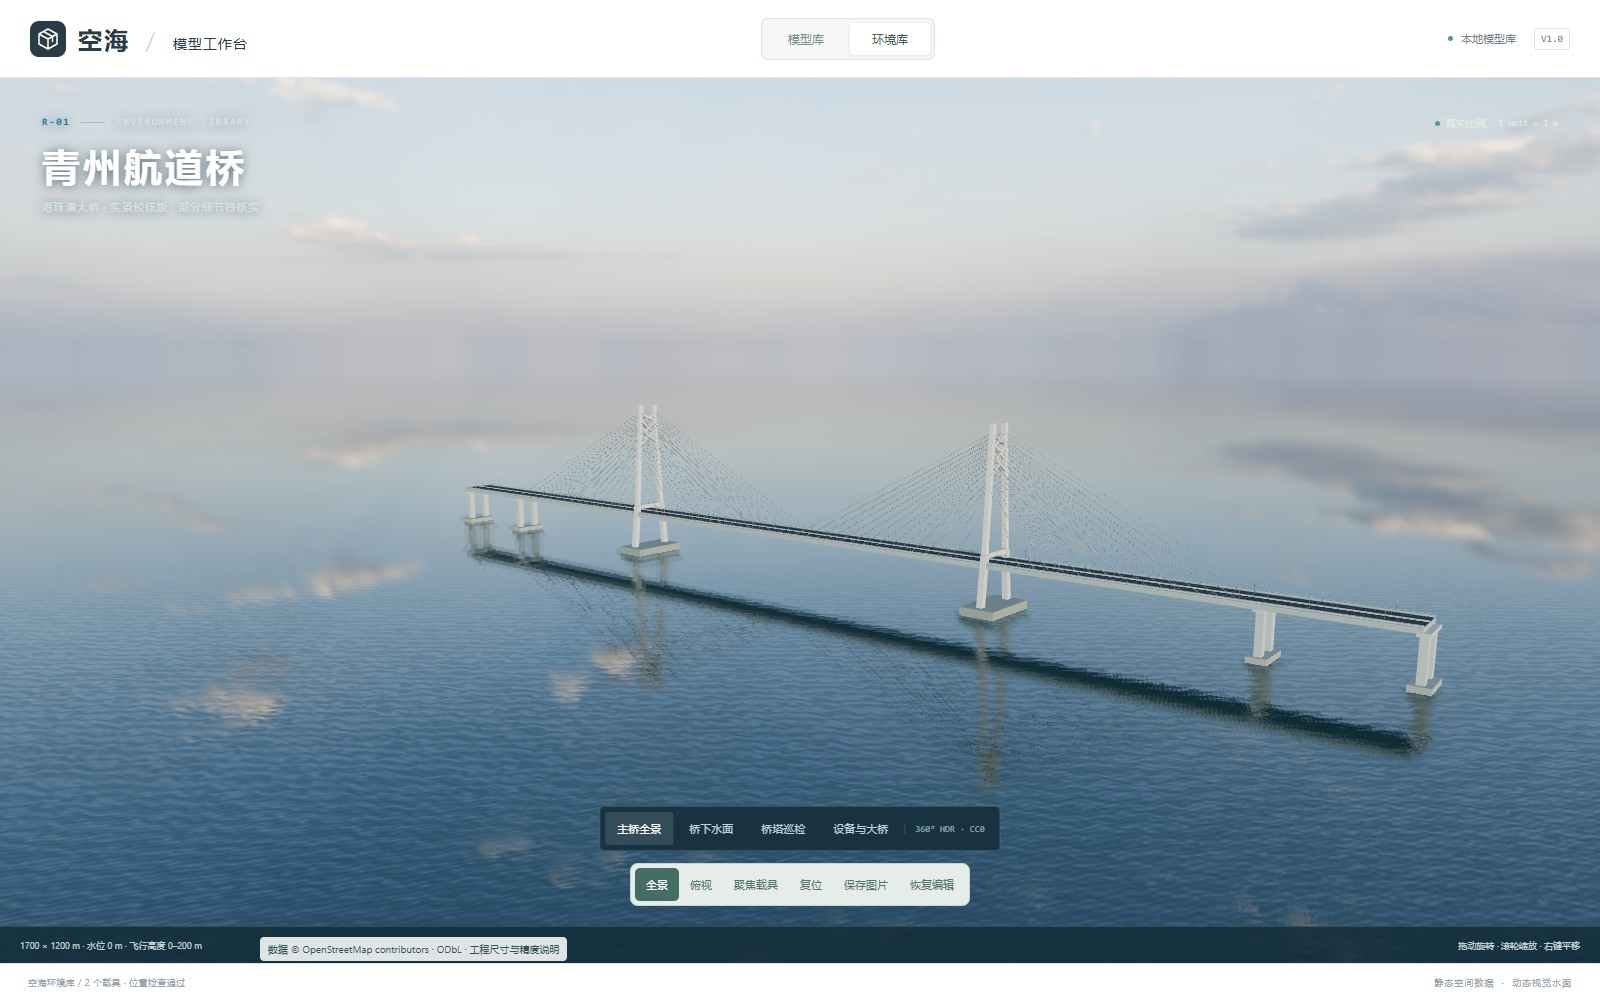
\includegraphics[width=.49\linewidth]{images/qingzhou.jpg}\hfill
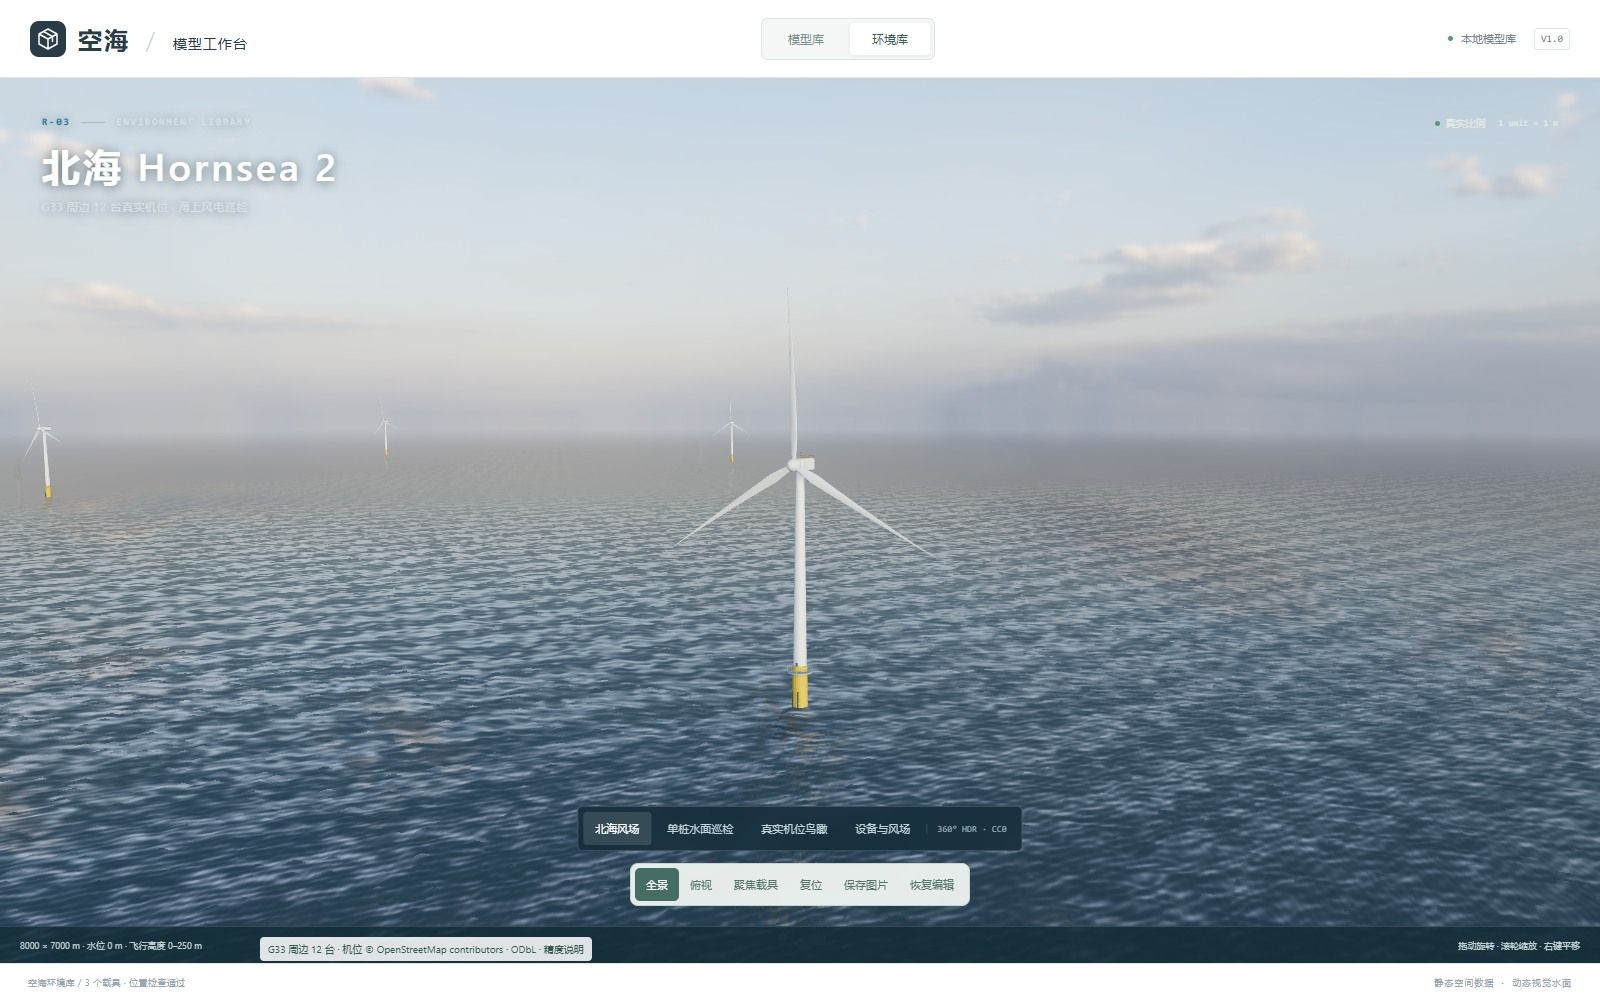
\includegraphics[width=.49\linewidth]{images/hornsea.jpg}
\caption{实景校核工程案例：（左）港珠澳大桥青州航道桥主跨与钻石型主塔；（右）英国北海 Hornsea 2 离岸风场 12 台真实机位。}
\end{figure}

\subsection{新增三大实景集群水域特征}
2026-10-24 扩充的西湖、加冷与瓦尔港场景，基于 OpenStreetMap 真实地理矢量轮廓裁剪构建：
\begin{itemize}
  \item \textbf{杭州西湖三岛水域（\texttt{westlake}）}：采用 UTM 51N（EPSG:32651）等距投影，岸高 2.2 m，严密保留三潭印月、湖心亭、阮公墩等岛屿孔洞。场景默认预置 12 艘 S-02 水文测量艇（4列 $\times$ 3行编队，间距 14 m），并内嵌 2 条 12 m 静态净空缓冲参考航线；
  \item \textbf{新加坡加冷盆地（\texttt{kallang}）}：采用 UTM 48N（EPSG:32648），岸高 2.5 m，包含 1443 个实际建筑轮廓（80个具有官方 OSM 高程），预置 3 条 8$\sim$12 m 净空走廊；
  \item \textbf{鹿特丹瓦尔港（\texttt{waalhaven}）}：采用 UTM 31N（EPSG:32631），岸高 3.2 m，复现 2176 个工业建筑与码头泊位，预置 3 条 15 m 宽阔纵深参考航线。
\end{itemize}

\begin{figure}[htbp]\centering
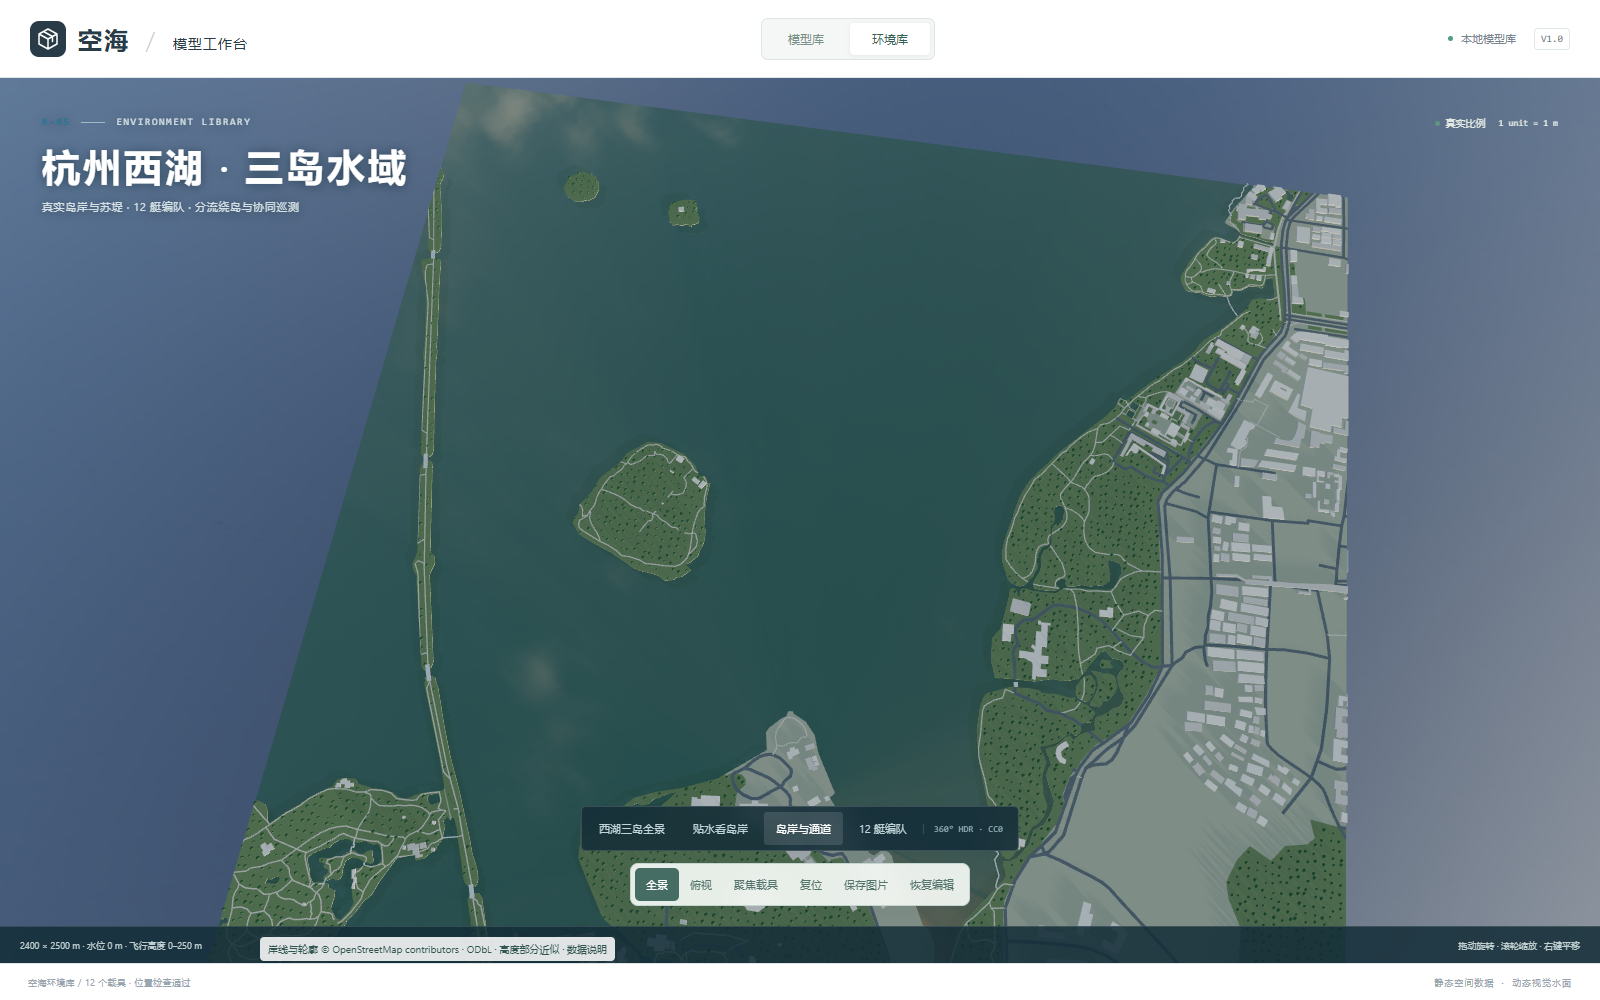
\includegraphics[width=.68\linewidth]{images/westlake.png}
\caption{杭州西湖三岛水域实景：真实湖岸、岛屿孔洞拓扑与 12 艘无人艇编队协同作业呈现。}
\end{figure}

\subsection{宏大空间尺度下的数值稳定性：对数深度缓冲}
在水平跨度达 $8000\,\text{m}$ 的大场景中，传统线性深度映射在远景会导致严重的 Z-fighting 闪烁。系统全管线适配\textbf{对数深度缓冲（Logarithmic Depth Buffer）}：
\begin{equation}
z_{\text{clip}} = \left[ \frac{\log(C \cdot z_{\text{view}} + 1)}{\log(C \cdot z_{\text{far}} + 1)} \cdot 2 - 1 \right] \cdot w_{\text{clip}}
\end{equation}
结合工程几何共面接缝微调与自定义水面着色器，消除了深水港与远景群岛环绕观察时的图元频闪。

\section{光度学对齐、大气散射与动态水面物理渲染}

系统构建了室外大尺度水域的光度学对齐闭环渲染管线，避免光影脱节的虚假“塑料感”。

\begin{center}
\begin{tikzpicture}[node distance=6mm, every node/.style={font=\small},
box/.style={draw=sea,rounded corners=3pt,fill=pale,text width=34mm,align=center,minimum height=12mm,line width=0.8pt},
arr/.style={-{Latex[scale=1.1]},thick,draw=sea}]
\node[box] (hdr) {\textbf{本地 2K HDR 全景}\\保留全动态辐射度跨度\\Poly Haven CC0};
\node[box,right=of hdr] (pmrem) {\textbf{PMREM 辐射度预过滤}\\生成粗糙度 mipmaps\\估算半球主光方向};
\node[box,right=of pmrem] (pbr) {\textbf{物理材质 PBR 着色}\\物体接收真实光照比\\同源方向光平行高光};
\node[box,below=of pmrem] (water) {\textbf{动态海面物理混合}\\平面裁剪反射 Reflector\\Schlick-Fresnel + 多尺度波纹};
\node[box,below=of pbr] (final) {\textbf{ACES Filmic 色调映射}\\曝光收敛至真实动态\\地平线颜色自适应大气雾};

\draw[arr] (hdr) -- (pmrem);
\draw[arr] (pmrem) -- (pbr);
\draw[arr] (pmrem) -- (water);
\draw[arr] (pbr) -- (final);
\draw[arr] (water) -- (final);
\draw[arr] (hdr.south) |- (final.west);
\end{tikzpicture}
\end{center}

\subsection{HDR 辐射度环境与主光源动态对齐}
采用 Poly Haven 的 \textit{Kloppenheim 06 Pure Sky} 本地 2K 高动态范围全景辐射图。通过 PMREM 预过滤生成多级漫反射与镜面反射贴图，并对 HDR 上半球纹理进行亮度能量积分扫描推算太阳方向：
\begin{equation}
\mathbf{d}_{\text{sun}} = \operatorname{normalize}\left(\arg\max_{(u, v) \in [0,1] \times [0.5,1]} L_{\text{hdr}}(u, v)\right)
\end{equation}
以此方向驱动主平行光并投射柔和阴影，确保物体受光面、水面镜向高光与天空云隙光在几何上严格共轴。

\subsection{动态海面混合与整数网格散列去噪}
定制水面着色器结合对称虚拟相机的 Planar Reflector 平面反射通道、多频法线扰动与 Schlick 近似 Fresnel 混合（$R_0 \approx 0.02$）。地平线处动态采样 HDR 边界色彩注入指数平方距离雾（\texttt{FogExp2}）。
针对贴水掠射视角曾出现的三角形杂影，系统将基于正弦波的浮点散列彻底重构为\textbf{整数网格置换散列（Integer Lattice Hash）}，彻底根治了浮点精度截断引发的三角面断层。

\shot{ninepin-waterline.jpg}{.68}{香港果洲群岛岛间水道：柱状节理岩岸、多载具编队、水面镜向反射与云天构成丰富纵深。}

\section{无人艇协同与运动规划算法库}

2026-10-24 系统正式发布了独立的无人艇运动规划与集群协同算法库（\texttt{src/algorithms/}），作为与三维渲染高度解耦的纯数学计算子系统，不仅可在 Web Worker 异步多线程执行，亦能与三维环境库无缝映射。

\subsection{五项核心规划与协同算法}
算法库集成了涵盖单艇导航与多艇编队的 5 类代表性算法：
\begin{enumerate}
  \item \textbf{A* 启发式最短路径规划}：在 8 邻接连续连通离散栅格上，采用欧氏距离启发式引导搜索：
  \begin{equation}
  f(n) = g(n) + h(n), \quad h(n) = \|\mathbf{p}_n - \mathbf{p}_{\text{goal}}\|_2
  \end{equation}
  结合基于视线投射（Ray-casting Line-of-Sight）的通视折线简化，在复杂岛礁水域剔除多余折点，生成几何平滑航迹；
  \item \textbf{Dijkstra 最短路径基准}：在完全相同的离散拓扑图上令 $h(n) \equiv 0$，对比展开规模。在西湖实测算例中，A* 仅展开 294 个节点即寻得最优路径，而 Dijkstra 展开 3725 个节点，两者的最终图代价严格一致（$928.89\,\text{m}$），严谨验证了启发式设计的算力收敛优势；
  \item \textbf{领航—跟随编队协同（Leader-Follower）}：领航艇跟踪 A* 路径，跟随艇采用分布式误差反馈控制律：
  \begin{equation}
  \mathbf{u}_i = \mathbf{u}_0 + k_p (\mathbf{p}_0 + \mathbf{d}_i - \mathbf{p}_i)
  \end{equation}
  实施单艇限速与队形自适应缩放，实验中队形跟踪误差快速收敛至 $10^{-13}\,\text{m}$ 精度；
  \item \textbf{分布式一致性编队控制（Consensus Formation）}：基于固定完全图拓扑，定义位移状态 $q_i = p_i - d_i$ 与控制律：
  \begin{equation}
  \mathbf{u}_i = k_c (\bar{\mathbf{q}} - \mathbf{q}_i), \quad \bar{\mathbf{q}} = \frac{1}{N} \sum_{j=1}^N \mathbf{q}_j
  \end{equation}
  保证质心不变性，初始队形偏移 50\% 条件下平稳收敛至 RMS 误差 $< 0.15\,\text{m}$；
  \item \textbf{分区往复全覆盖搜索（Partitioned Reciprocal Coverage）}：针对指定矩形水域实施沿主轴均分切片，多艇独立执行梳状条带遍历；遇到岛屿或岸线障碍时，局部自适应调用 A* 算法动态拼接绕行动作，实测采样点覆盖率达 100\%。
\end{enumerate}

\begin{figure}[htbp]\centering
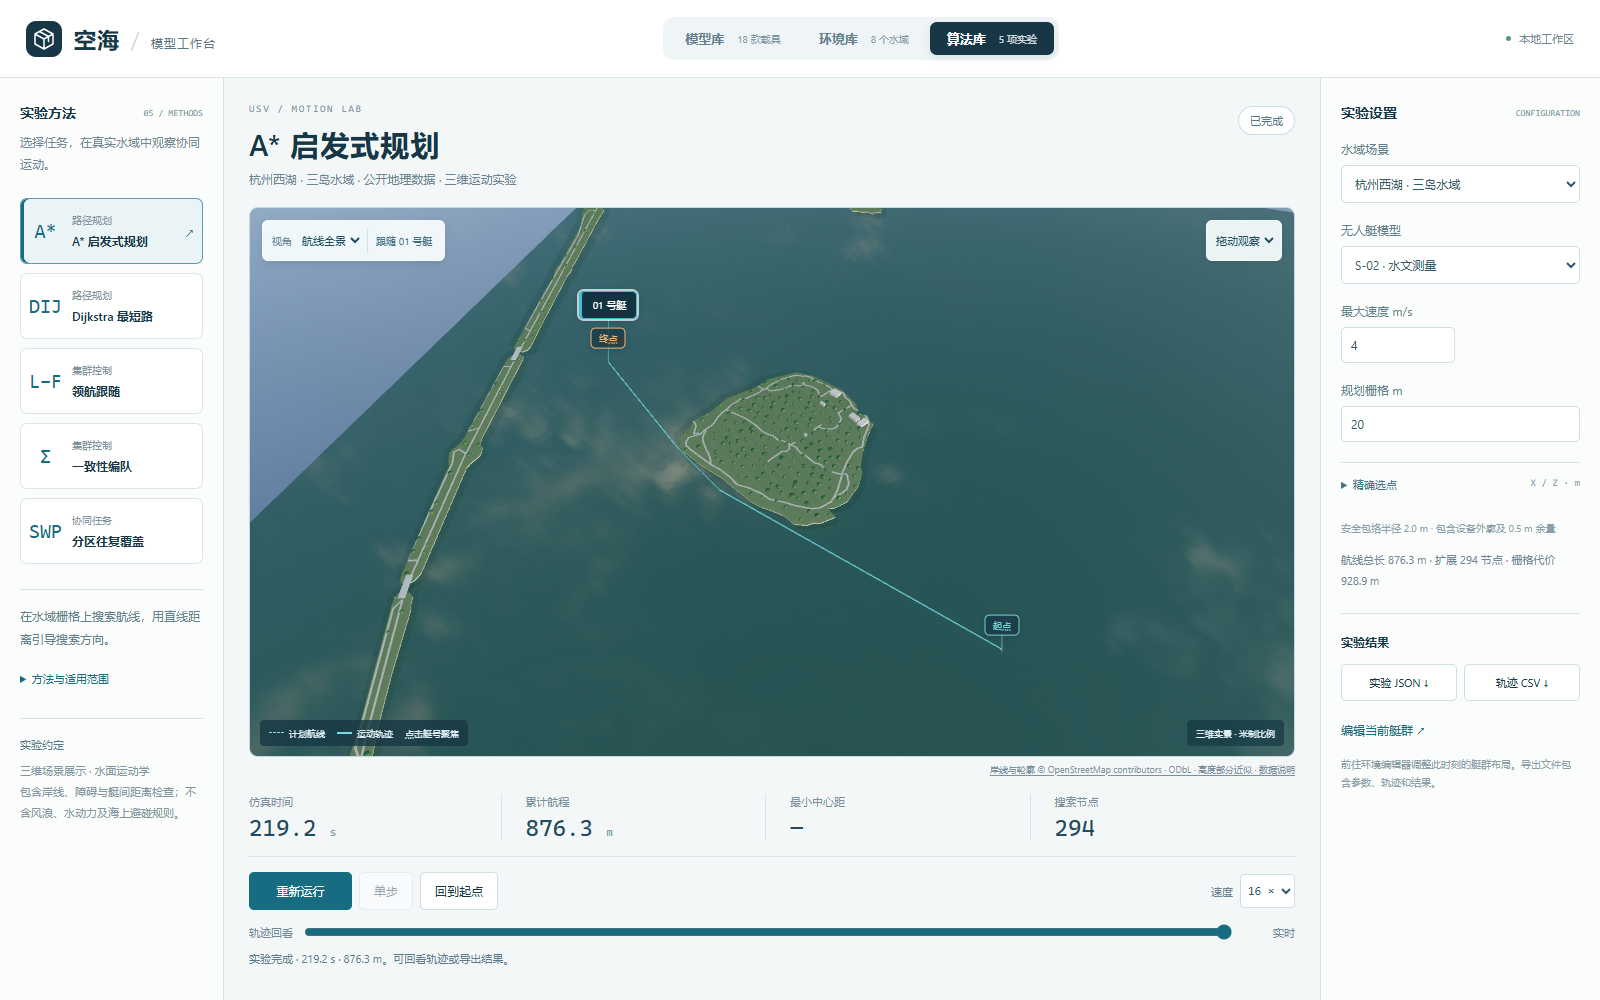
\includegraphics[width=.49\linewidth]{images/astar.png}\hfill
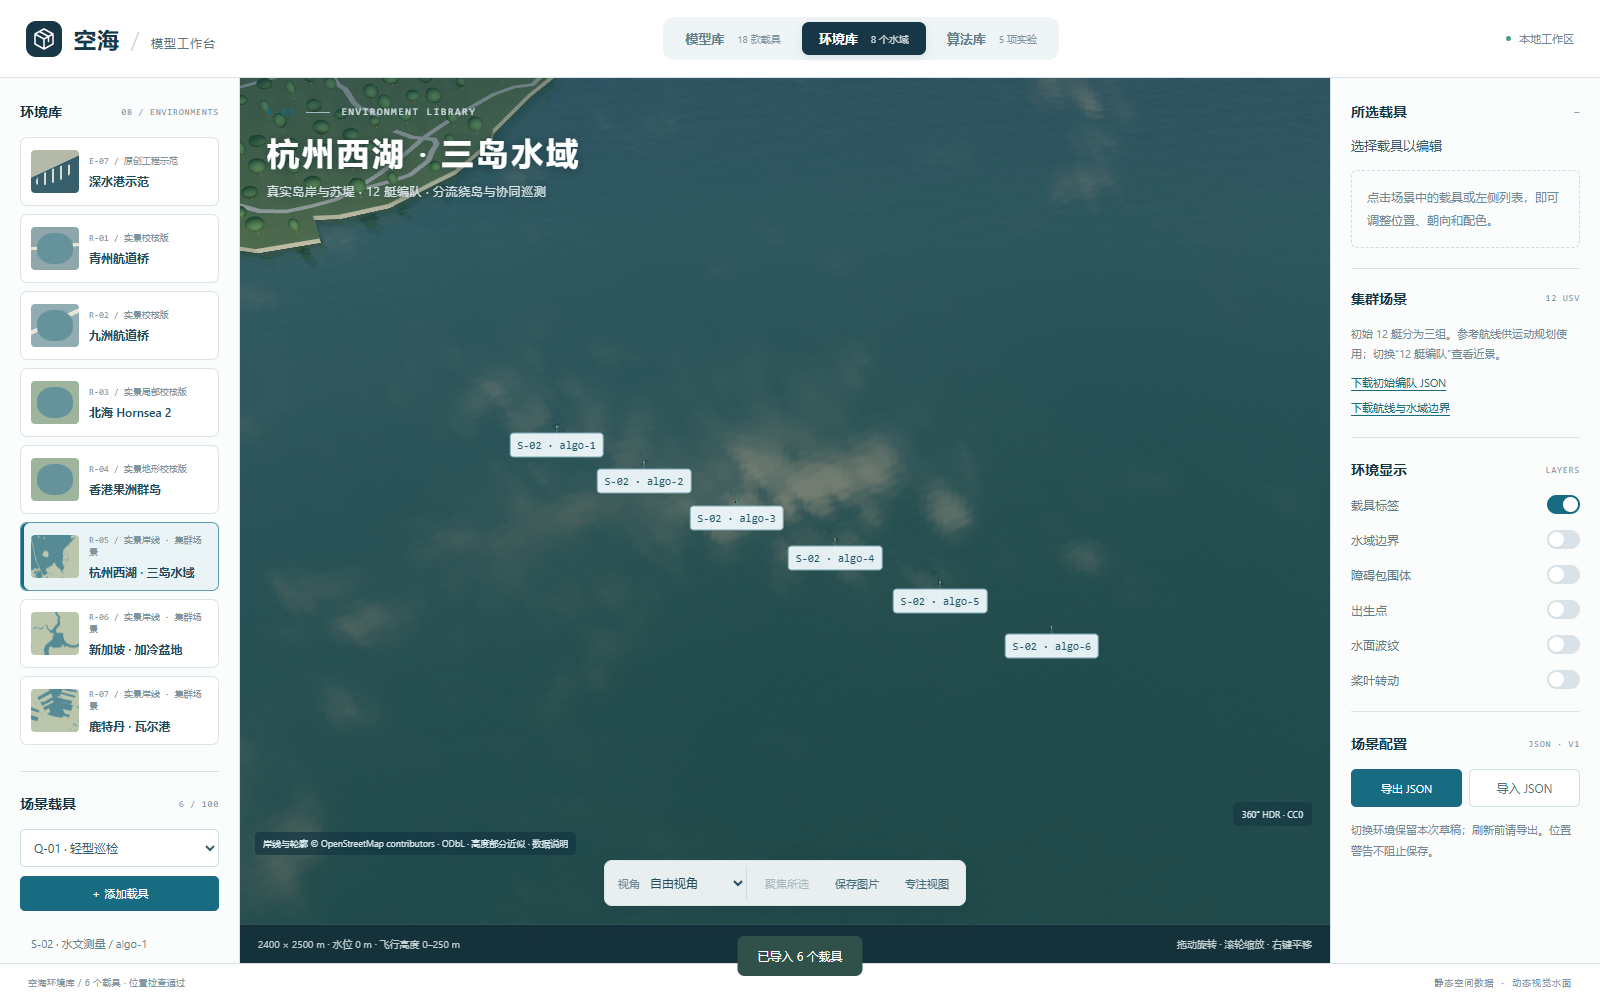
\includegraphics[width=.49\linewidth]{images/coverage.png}
\caption{算法库实验与三维映射：（左）A* 在杭州西湖三岛水域的绕岛最短路径；（右）多艇分区往复覆盖快照一键映射至三维真实场景。}
\end{figure}

\subsection{连续碰撞门（Continuous Collision Gate）与防穿透安全}
仿真系统摒弃了仅在时间离散点检查位置的传统缺陷，引入了基于线段扫掠体与相对运动速度的连续碰撞检测门：
\begin{equation}
\mathcal{C}_{\text{swept}} = \left\{ \mathbf{x} \in \mathbb{R}^2 \;\middle|\; \operatorname{dist}\left(\mathbf{x}, \overline{\mathbf{p}(t)\mathbf{p}(t+\Delta t)}\right) \le R_{\text{safe}} \right\}
\end{equation}
同时计算两艇之间的相对运动线段最小间距。若相对距离小于安全阈值，强制截断发生冲突的动作，并级联复核停机引发的新冲突，彻底杜绝了大步长运动下的穿透（Tunnelling）事故。

\subsection{二维仿真与三维场景跨空间双向联动}
算法库设计了完备的科研交互与数据管线：
\begin{itemize}
  \item \textbf{时间轴轨迹回看（Scrubbing）}：支持 1x/4x/16x/32x 倍速播放、暂停与 0.1s 单步步进，任意时刻可拖动滑块查看历史帧；
  \item \textbf{三维环境库快照映射}：点击“在环境库中查看当前艇群”，可将二维算法在任意时刻的集群位置与偏航角（Yaw）原子化打包为符合环境库标准的场景配置文件，直接在 WebGL 中观察真实模型姿态；
  \item \textbf{标准科研数据导出}：支持导出包含全量参数与计划的 JSON，以及时序轨迹 CSV 文件（格式为 \texttt{time\_s,vessel\_id,x\_m,z\_m,yaw\_rad}）。
\end{itemize}

\section{全链路工程验收、性能基准与实测分析}

系统恪守“以可重复、可度量的自动化测试约束视觉判断”之工程准则，全量功能均纳入自动化回归体系。

\subsection{自动化回归测试矩阵（31 项全量通过）}
\begin{table}[H]\centering\small
\begin{tabularx}{\linewidth}{@{}llX@{}}\toprule
验收模块 & 覆盖范围 & 核心断言与通过标准\\\midrule
算法单元测试 & \texttt{tests/algorithms.test.ts} & A* 与 Dijkstra 最优代价一致性；凸孔障碍扫掠防穿透；一致性收敛性；覆盖率 100\%\\
模型单元测试 & \texttt{tests/models.test.ts} & 18 款模型有限坐标；单尖船首流形水密性；旋翼数严格为 4；独立释放\\
环境单元测试 & \texttt{tests/environments.test.ts} & 8 大水域几何有限性；高低空障碍高程解耦；确定性随机种子生成\\
集群水域测试 & \texttt{tests/usv-sites.test.ts} & 西湖/加冷/瓦尔港 OSM 矢量水陆拓扑闭合；12 艇编队安全净空；参考航线走廊覆盖\\
静态构建审查 & TypeScript / Vite & \texttt{tsc --noEmit} 零报错；模块间依赖循环严格为零\\\bottomrule
\end{tabularx}
\caption{工程验收与自动化质量保证测试矩阵汇总表（31 项测试全量通过）。}
\end{table}

\shot{workbench.jpg}{.68}{中文交互式三维模型工作台：支持 18 款载具实时装配、环绕检视、参数化微调与状态快照保存。}

\subsection{真实硬件性能剖析基准}
性能基准在搭载 Intel Arc 140V GPU 的测试节点上通过 Edge 无头浏览器实测采集（渲染画布 $1600 \times 1000$，$\text{DPR} = 1$），场景内布设 12 艘无人艇集群：
\begin{itemize}
  \item \textbf{高密度集群帧率与帧间隔}：在西湖、加冷与瓦尔港实景水域工况下，平均帧率稳定于 $58\text{--}60\,\text{FPS}$，平均帧间隔为 $16.67\,\text{ms}$，P95 间隔稳定在 $16.8\text{--}16.9\,\text{ms}$；
  \item \textbf{显存幂等释放与资源泄漏审计}：在连续 3 轮执行新增实景水域场景的完全销毁与重建循环后，WebGL 上下文中的活动几何体（Geometry）数量恒定收敛于 1275，活动纹理（Texture）恒定收敛于 18，彻底阻断了显存漂移。
\end{itemize}

\subsection{科学边界与局限性声明}
本系统侧重于空间拓扑、几何约束、工程布局与光度学表现的实时呈现，\textbf{尚未实装}计算流体动力学（CFD）、高精度水动力六自由度（6-DOF）非线性波浪耦合、实测水下多波束测深高程与海上避碰规则（COLREGs）；部分建筑高度为规则估算，桥位按水面保守障碍处理。

\section{开源治理、复现指南与演进路线}

\subsection{全本地化可重现构建指南}
系统运行完全基于本地资源，\textbf{绝不发起任何外部在线地图底图请求或商业云端 API 交互}。完整复现指令如下：

\begin{lstlisting}
# 1. 安装项目锁定依赖并启动本地三维实时服务
npm ci
npm run dev

# 2. 执行全量 31 项单元测试与生产构建
npm test
npm run build

# 3. 执行集群水域与算法库无头浏览器自动化验收
npm run test:usv-sites
npm run test:algorithms

# 4. 编译高质量 XeLaTeX 中文技术白皮书
cd docs/development-log
xelatex -interaction=nonstopmode -halt-on-error main.tex
xelatex -interaction=nonstopmode -halt-on-error main.tex
\end{lstlisting}

\subsection{第三方数据合规与知识产权台账}
\begin{table}[H]\centering\small
\begin{tabularx}{\linewidth}{@{}llX@{}}\toprule
资产类别 & 权利人 / 机构 & 许可协议与合规使用声明\\\midrule
天空全景辐射图 & Greg Zaal / Jarod Guest / Poly Haven & CC0 1.0 Universal 公有领域贡献声明，本地打包集成商用\\
地理矢量岸线与机位 & OpenStreetMap 贡献者 & 遵循 Open Database License (ODbL) 1.0，明确保留署名与原始 ID\\
数字地形模型（DTM） & 香港特别行政区政府地政总署 & 经 DATA.GOV.HK 开放获取，严格遵守其条款并保留衍生转换说明\\
工程研究参考影像 & 中建、上港、Ørsted、Arup、新华社等 & 仅作为学术研究比对超链接，不随代码库分发，不作商用材质贴图\\
核心工程代码库 & 朱华天、Gemini 3.8 Flash、GPT-6 Astra & 遵循宽松 MIT 开源许可证，允许科研学术自由分发与二次衍生\\\bottomrule
\end{tabularx}
\caption{项目知识产权、第三方数据源与开源许可证合法性合规台账。}
\end{table}

\subsection{未来技术演进路线}
后续工作将聚焦于：(1) 跨介质多载具流固耦合与六自由度（6-DOF）水动力学浮态解算；(2) 离岸风机尾流效应与低空微气象扰动场建模；(3) 结合水文多波束测深实测点云的水下声呐仿真。

\section*{参考文献与资源溯源}
\begin{enumerate}\small
\item 项目公开代码仓库：\url{\repo}。
\item 高动态范围天空素材：\href{https://polyhaven.com/a/kloppenheim_06_puresky}{Poly Haven, Kloppenheim 06 Pure Sky}，遵循 CC0 1.0 协议。
\item OpenStreetMap 开放地理数据版权与法律声明：\url{https://www.openstreetmap.org/copyright}。
\item 香港特别行政区政府地政总署：\href{https://data.gov.hk/en-data/dataset/hk-landsd-openmap-5m-grid-dtm}{5 米网格数字地形模型（DTM）}，使用条件详见 DATA.GOV.HK 条款。
\item P. E. Hart, N. J. Nilsson, B. Raphael, ``A Formal Basis for the Heuristic Determination of Minimum Cost Paths,'' \textit{IEEE Transactions on Systems Science and Cybernetics}, 1968.
\item E. W. Dijkstra, ``A note on two problems in connexion with graphs,'' \textit{Numerische Mathematik}, 1959.
\item R. Olfati-Saber, R. M. Murray, ``Consensus Problems in Networks of Agents With Switching Topology and Time-Delays,'' \textit{IEEE Transactions on Automatic Control}, 2004.
\item H. Choset, P. Pignon, ``Coverage Path Planning: The Boustrophedon Decomposition,'' \textit{Field and Service Robotics}, 1997.
\item 项目工程溯源台账及环境架构技术细节：详见仓库各工程说明文档及 \texttt{sources.json} 台账。
\end{enumerate}

\vfill
\noindent{\color{sea}\rule{\linewidth}{0.6pt}}
\vspace{1mm}
\noindent{\small\color{muted}本技术白皮书系统总结了截至 2026年10月24日“空海”跨介质素材库的工程架构、理论模型、集群场景与运动规划算法体系。它既作为程序化三维建模与真实地理仿真的开发记录，亦为跨介质机器人仿真、智能感知与多智能体协同控制算法提供了高可靠性的数字基座。}

\end{document}
